\section{Audio and Heartbeat} 
\label{audio_and_heartbeat}
The audio and heartbeat system runs concurrently with the rest of the program. On an operating system supporting neither multi-processes nor threads this means using interrupts to stop normal execution and perform tasks on the side.\\
\par
The idea is to configure the hardware to trigger a hardware interrupt at a regular interval. This interrupt is caught by a system called PIC which transforms it into a software interrupt. The software interrupt ID is used as an offset in a vector to look up a function belonging to the engine. At this point, the CPU is stopped (a.k.a: interrupted) from doing whatever it was doing (likely running the 3D renderer), and it starts running the interrupt handler which is called an ISR\footnote{Interrupt Service Routine}. We now have two systems running in parallel.\\
\par
\begin{figure}[H]
  \centering
  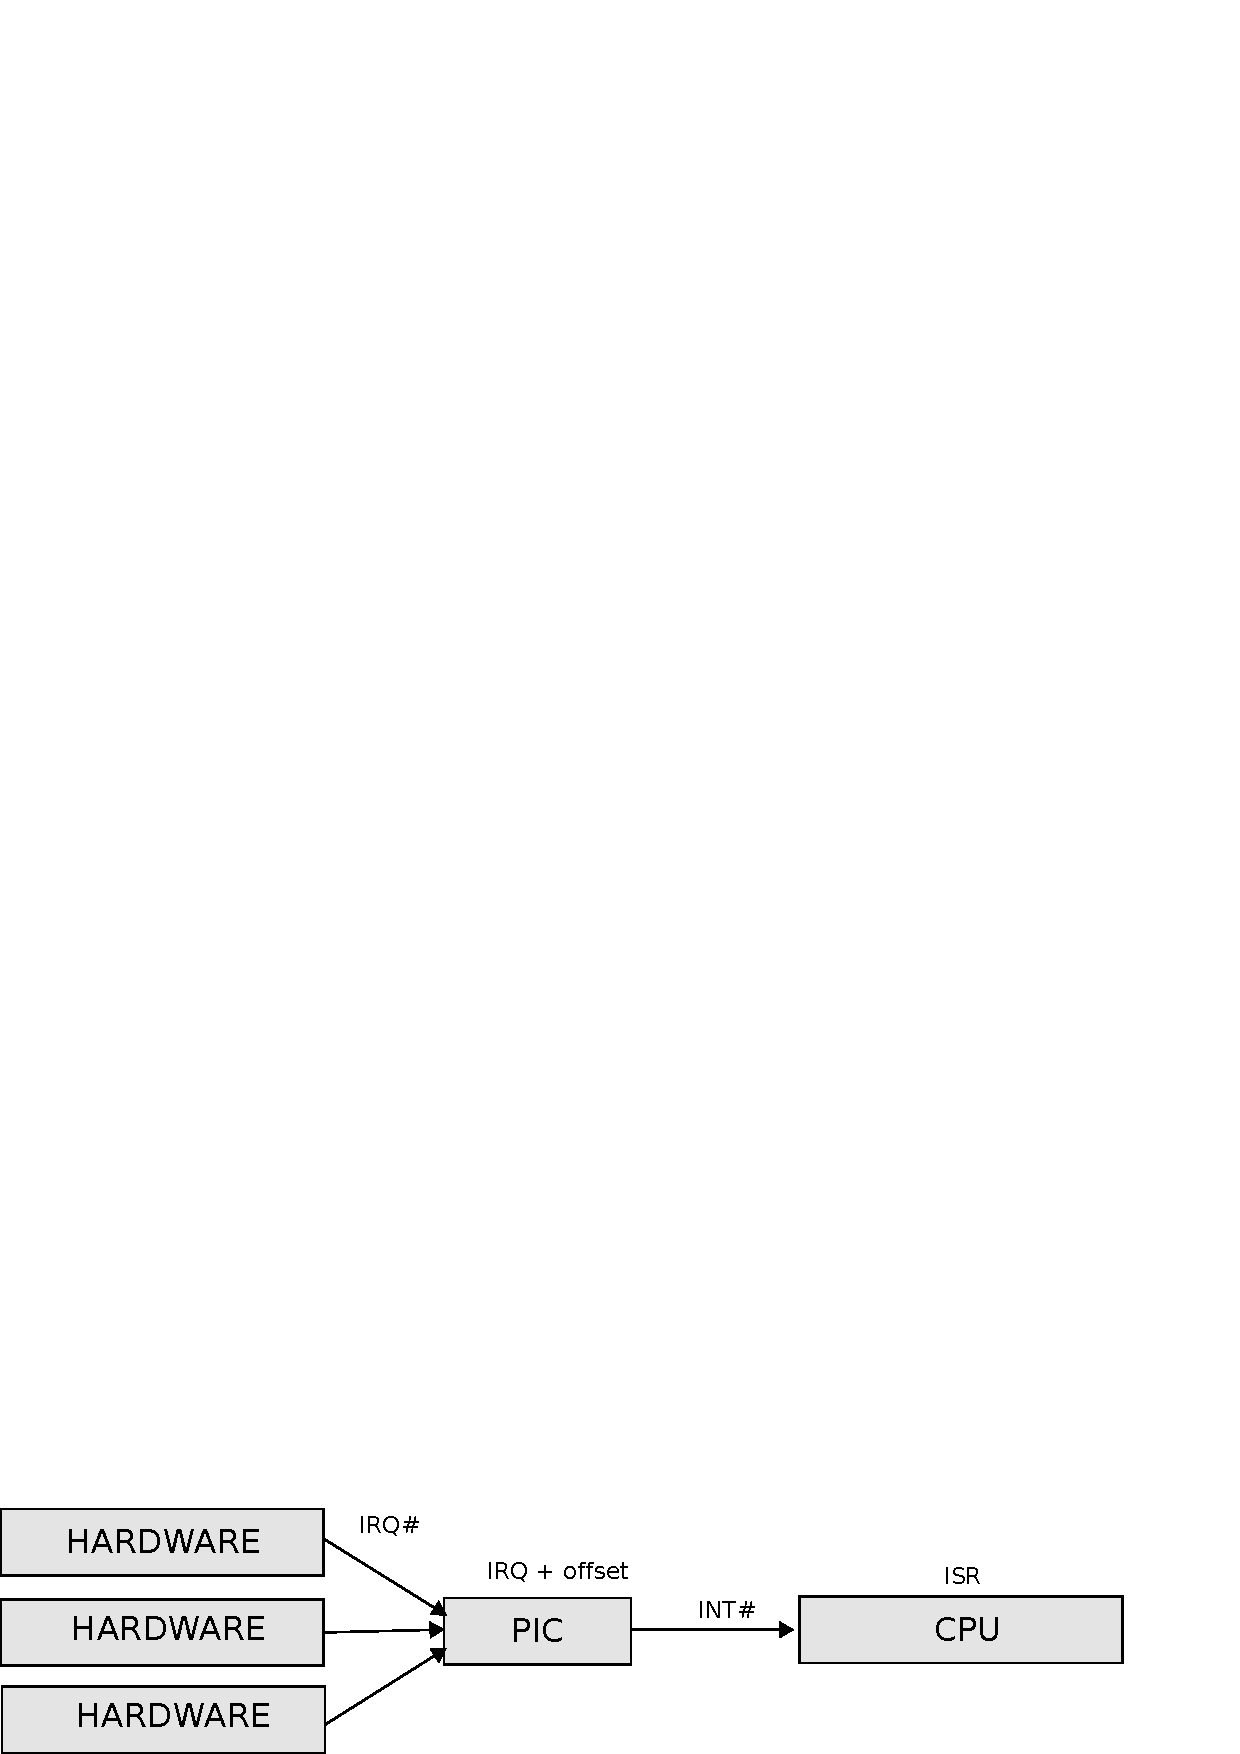
\includegraphics[width=\textwidth]{imgs/drawings/irqs/explanationsvg.pdf}
  \caption{Hardware interrupts are translated to software interrupt via the PIC.}
\end{figure}
\par
 Since interrupts keep triggering constantly from various sources, an ISR must choose what should happen if an IRQ is raised while it is still running. There are two options.  The ISR can decide it needs a "long" time to run and disable other IRQs via the IMR \footnote{Interrupt Mask Register}. This path introduces the problem of discarding important information such as keyboard or mouse inputs.\\
 \par
 Alternately, the ISR can decide not to mask other IRQs and do what it is supposed to do as fast as possible so as to not delay the firing of other important interrupts that may lose data if they aren't serviced quickly enough.\\
 \par
 Wolfenstein 3D uses the latter approach and keeps tasks in its ISR very small and short. To this effect everything in the audio and heartbeat system is written in assembly and avoids "heavy" processing.

\subsection{IRQs and ISRs}
The IRQ and ISR system relies on two chips: the Intel 8254 which is a PIT \footnote{Programmable Interval Timer} and the Intel 8259 which is a PIC \footnote{Programmable Interrupt Counter}. The PIT features a crystal oscillating in square waves. On each period, it decrements its three counters. Counter \#2 is connected to the RAM in order to automatically perform something called "memory refresh"\footnote{Without frequent refresh, DRAM will lose its content. This is one of the reasons it is slower and SRAM is preferred in the caching system.}. Counter \#1 is connected to the buzzer and generates sounds. Counter \#0 is connected to the PIC. When counter \#0 hits zero it generates an IRQ\footnote{Interrupt Request Line: Hardware lines over which devices can send interrupt signals to the CPU.} and sends it to the PIC.\\
\par
\begin{figure}[H]
  \centering
  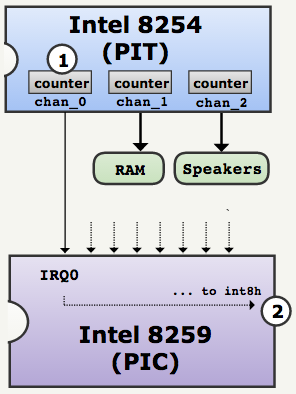
\includegraphics[width=.65\textwidth]{imgs/drawings/heatbeats.pdf}
  \caption{Interactions between PIT and PIC.}
\end{figure}
\par

The PIC's hardware IRQ-0 to IRQ-8 are mapped to the Interrupt Vector starting at Offset 8 (resulting in mapping to software interrupts INT08 to INT0F). \pagebreak

\begin{figure}[H]
	\centering
	\begin{tabularx}{\textwidth}{ l p{.5\textwidth}  }
	  \toprule
	  \textbf{I.V.T Entry \#} & \textbf{Type} \\ \bottomrule

	  00h	&	CPU divide by zero \\
01h	&	Debug single step \\
02h	&	Non Maskable Interrupt \\
03h	&	Debug breakpoints \\
04h	&	Arithmetic overflow \\
05h	&	BIOS provided Print Screen routine \\
06h	&	Reserved \\
07h	&	Reserved \\

		08h & IRQ0, System timer \\
		09h & IRQ1, Keyboard controller \\
		0Ah & IRQ2, Bus cascade services for second 8259 \\
		0Bh & IRQ3, Serial port COM2 \\ 
		0Ch & IRQ4, Serial port COM1 \\
		0Dh & IRQ5, LPT2, Parallel port 2 \\
		0Eh & IRQ6, Floppy Disk Controller \\
		0Fh & IRQ7, LPT2, Parallel port 1 \\
		10h & Video services (VGA)\\
		11h & Equipment check \\
		12h & Memory size determination \\
		%13h & ATA channel 1 \\
		%14h & ATA channel 2  \\
		\bottomrule
	\end{tabularx}
	\caption{The Interrupt Vector Table (entries 0 to 18).}
\end{figure}
Notice \#8 which is associated with the System timer and usually updates the operating system clock. Because IVT \#8 was hijacked, the operating system clock is not updated while Wolfenstein 3D runs. Upon exiting the game, DOS will run late by the amount of time played.\\
\par
Using these two chips and placing its own function at Interrupt Vector Table (IVT) \#8, the engine can stop its runtime at a regular interval, effectively implementing a subsystem running concurrently with everything else.\\
\par
The engine can decide at what frequency to be interrupted, depending on the type of sound/music it needs to play and what devices will be used. As a result, three different ISRs can be found at IVT \#8: 
\begin{enumerate}
\item \cw{SDL\_t0SlowAsmService} when running at 140Hz, to play sound effects on the beeper via PWM and PCM audio effects on SoundBlaster.
\item \cw{SDL\_t0FastAsmService} when running at 700Hz, to play FM music, FM sound effects on AdLib, and PCM audio effects on Disney Sound Source.
\item \cw{SDL\_t0ExtremeAsmService} when running at 7000Hz, to play PCM sound in an alternate way. This mode was never enabled in shipping products (see page \pageref{pcs_pcm}).
\end{enumerate}
\par



\subsection{PIT and PIC}
The PIT chip runs at 1.193182 MHz. This initially seems like an odd choice from the hardware designers, but has a logical origin. In 1980 when the first IBM PC 5150 was designed, the common oscillator used in television circuitry was running at 14.31818 MHz. As it was mass produced, the TV oscillator was very cheap so utilizing it in the PC drove down cost. Engineers built the PC timer around it, dividing the frequency by 3 for the CPU (which is why the Intel ran at 4.7Mhz), and dividing by 4 to 3.57Mhz for the CGA video card. By logically ANDing these signals together, a frequency equivalent to the base frequency divided by 12 was created. This frequency is 1.1931816666 MHz. By 1991, oscillators were much cheaper and could have used any frequency but backward compatibility prevented this.\\
\par














\subsection{Heartbeats}
Each time the interrupt system triggers, it runs another small (yet paramount) system before taking care of audio requests. The sole goal of this heartbeat system is to maintain a 64 bit variable: \cw{TimeCount}.\\
\par
\begin{minipage}{\textwidth}
\lstinputlisting[language=C,morekeywords={longword}]{code/timecount.c}
\end{minipage}
\par
It is updated at a rate of 70 units per seconds (to match the VGA update rate of 70Hz). These units are called "ticks". Depending on how fast the audio system runs (from 150Hz to 7000Hz), it adjusts how much it should increase \cw{TimeCount}.\\
\par
Every system in the engine uses this variable to pace itself. The renderer will not start rendering a frame until at least one tick has passed. The AI system expresses action duration in tick units. The input sampler checks for how long a key was pressed, and the list goes on... Everything interacting with human players uses \cw{TimeCount}.\\













\subsection{Audio System}
The audio system is complex because of the fragmentation of audio devices it can deal with. The early 90s was a time before Windows 95 harnessed all audio cards under the DirectSound common API. Each development studio had to write their own abstraction layer and id Software was no exception. At a high level, the Sound Manager offers a lean API divided in two categories: one for sounds and one for music.\\
\par
\begin{minipage}{\textwidth}
\lstinputlisting[language=C,morekeywords={longword}]{code/sound1.h}
\end{minipage}
\par
\begin{minipage}{\textwidth}
\lstinputlisting[language=C,morekeywords={longword}]{code/sound.h}
\end{minipage}
\par
\vspace{10pt}
But in the implementation lies a maze of functions directly accessing the I/O port of four sound outputs: AdLib, SoundBlaster, Buzzer, and Disney Sound Source. All belong to one of the three supported families of sound generators: FM Synthesizer (Frequency Modulation), PCM (Pulse Code Modulation) or PWM (Pulse Width Modulation).\\


\subsection{Music}
Playing music is not too messy since only PCs equipped with a Yamaha YM3812 FM synthesizer could play tracks (a.k.a: with an AdLib or a SoundBlaster inside). As SoundBlaster made its programming interface compatible with AdLib there is only one code path to both cards. There is not a lot of magic here since this uses a piece of well-designed hardware dedicated to this specific task. There are a few cool tricks, though.\\
\par
The music system streams data to the sound cards. Music in the 90s was not in digitized formats like today's CD or MP3 formats (that would have taken too much storage space and bandwidth). Instead music was stored as series of notes played on channels simulating instruments. The format used is close to the notorious MIDI but with a few variations and is called IMF\footnote{Id Music Format}. It is proprietary to id Software and designed with OPL2 in mind (the raw format is exactly what is sent to the AdLib/Soundblaster synthesizer with no transformations). IMF has a hardcoded playback rate and music notes are played at 700 Hz.\\
\par
Hardware limitations dictated certain aspects of music design. The FM synthesizer (OPL2) has 9 channels (a.k.a instruments) yet the composer, Bobby Prince, was asked to use only channels 1 to 8. This little trick allows for multiplexing music and sound effects on AdLib cards since it leaves channel 0 available at all times (the SoundBlaster plays sound differently).\\




\subsubsection{OPL2/YM3812 Programming}
\label{IMF_explanation}
\par
Programming the OPL2 output is esoteric to say the least. AdLib and Creative did publish SDKs but they were expensive.  Documentation was sparse and often cryptic. Today, they are almost impossible to find.\\
\par
The OPL2 is made of 9 channels capable of emulating instruments. Each channel is made of two oscillators: a Modulator whose outputs are fed into a Carrier's input. Each channel has individual settings including frequency and envelope (composed of attack rate, decay rate, sustain level, release rate, and vibrato). Each oscillator can also pick a waveform (these characteristic forms are what gave the YM3812 its recognizable sound).\\
\par
 To control all of these channels, a developer must configure the OPL2's 244 internal registers. These are all accessed via two external I/O ports. One port is for selecting the card's internal register and the other is to read/write data to it.\\
\par
\begin{minipage}{\textwidth}
\lstinputlisting[language=C,morekeywords={longword}]{code/audio_ports.c}
\end{minipage}
\par
When the AdLib was released in 1986, developers were instructed to send data "as fast as possible". At 4.77Mhz, a PC was unable to out-pace the AdLib. Yet as CPUs got faster, issues started to arise and the card was unable to keep up.\\
\par

\begin{fancyquotes}
The original AdLib manual (before they shipped) did not call for ANY delays. The original IBM PC (4.77 Mhz) couldn't get ahead of the card. By the time it shipped they were telling use to do one IN instruction, and every time a new faster processor came out they added some delay to their recomendation. The old 8088 machines would not have worked with the 35 IN instructions now required, it would have slowed the machine down so much nothing else could get done.\\
 \par
 \textbf{Jason Linhart}
 \end{fancyquotes}
\\
\footnotetext{http://www.oldskool.org/guides/oldonnew/sound .}
\par
Later the Programming Guide was amended with reliable specs.\\
\par
\begin{fancyquotes}
Wait three point three (3.3) microseconds for the address, and twenty-three (23) microseconds for the data.\\
\par
\textbf{AdLib manual}
 \end{fancyquotes}
 

\par
The engine does not know about any of the details of the OPL2. There is zero abstraction layer or transformation here. An IMF song is made of a series of messages containing exactly the values to write to the register and data ports of the OPL2. Each message is four bytes:\\
\par
\begin{minipage}{\textwidth}
\lstinputlisting[language=C,morekeywords={longword}]{code/adlib_message.c}
\end{minipage}
\par
The \cw{reg} byte is sent to port \cw{0x388}, the \cw{data} byte is sent to \cw{0x389}, and the \cw{delay} 2 bytes are used to tell how much time to wait before sending the next register/data to the card. The stream is hard-coded at 700Hz and the delay is expressed in this unit: a value of 700 means to wait 1000ms before sending another command. Whenever there is music playing the engine runs at no less than 700Hz. A value of zero means the next message should be sent immediately.\\
\par
Overall, music is simple to execute because almost everything has been pre-processed via IMF. Every time the audio system wakes up, it checks if music packets should be sent, sends them, and moves on to the sound effects.










\section{Sound Effects}
Sound effects are where things become complicated. None of the cards use the same format and audio configurations are numerous. The sound settings screen, featuring now less than three sections illustrates how complex this is.\\
\par
\trivia{Notice how the sound settings screen on next page overlap. It is possible to select "SoundBlaster" twice in the SFX sections since it appears both in section "Sound Effects" and in section "Digitized Sound". It is far from obvious what to expect if such a configuration is selected.}\\
\par

 \cfullimage{audio/audio_settings.png}{Overlapping audio settings.}
\par
Sounds are stored in three formats.
\begin{enumerate}
\item PC Speaker.
\item AdLib.
\item SoundBlaster/Disney Sound Source.
\end{enumerate}
They are all package in the \cw{AudioT} archive created by Muse. Sounds are segregated by format but always stored in the same order. This way a sound can be accessed in three formats by using \cw{STARTPCSOUNDS} + \cw{sound\_ID} or \cw{STARTADLIBSOUNDS} + \cw{sound\_ID}.\\
\par
Strangely, only PC speaker and AdLib sounds are stored in the \cw{AUDIOT.*} files; the digitized sounds are in the \cw{VMSWAP.*} archive. As a result, offset \cw{STARTDIGISOUNDS} is never used. The authors of this code were asked, but it seems nobody can remember why.\\
\par
\begin{minipage}{\textwidth}
\lstinputlisting[language=C,morekeywords={longword}]{code/muse_header.c}
\end{minipage}
\pagebreak




\subsection{Sound Effects: AdLib}
AdLib only has an FM synthesizer, with sounds played on its Channel 0. Sounds are played the same way as music via IMF, as previously described.\\












\subsection{Disney Sound Source System: PCM}

The Disney Sound Source is simple to program\footnote{The Programmer's Guide to the Disney Sound Source is a whopping 2 pages!} because it can do only one thing. It plays  8 bit PCM audio at 7000Hz on a single channel. That's it -- nothing more, nothing less. Data is fed through the parallel port to the device, which is stored into a 16-byte FIFO queue, which then feeds an 8-bit DAC connected to its integrated loudspeaker.\\ 
\par
Even though the sampling rate is 7000Hz, the sound system needs not to run at such a high frequency. The 16 byte buffer allows to run at 700Hz and send a batch of 9-10 bytes every iterations. Every time the audio system wakes, it reads the DAC status to check how many bytes have been consumed in the FIFO. The engine pushes as many bytes as possible until the FIFO is full and returns. When the FIFO empties, the Disney Sound Source stops making noise.\\
\par










\par
\subsection{SoundBlaster System: PCM}
Since the SoundBlaster also supports 7000Hz PCM, it uses the same sound effects files as the Disney Sound Source. However, it also features a DSP which is DMA capable. As a result, the CPU does not have to waste cycles transferring data. The audio system has little to do and can allow itself to run in "slow" mode at 140Hz. It wakes up to point the DMA to the right memory address each time it crosses the end of a 16K segment via a DMA routine callback.\\
\par








\par
\subsection{SoundBlaster Pro System: Stereo PCM}
\par

On a "high-end" SoundBlaster Pro, the Mixer described on page \pageref{sbmixerpage} is used to simulate 3D sounds. The source of the sound is first rotated with the same formula seen on page \pageref{rotatematrix}. The player's position is used to generate two attenuation values (between 0 and 15) which are then packed in a byte and sent to the mixer. The difference in volumes tricks the player into perceiving the sound origin anywhere within the 180 degrees facing her.\\
\par 
\begin{minipage}{\textwidth}
\lstinputlisting[language=C]{code/setposition.c}
\end{minipage}
\par
\bu{Trivia :} Plugging in a SoundBlaster card was not enough to produce sound. This was before "plug \& play" was introduced by Windows 95. The user had to write a special line in the startup command of the PC (\cw{autoexec.bat}).\\
\par 
\begin{minipage}{\textwidth}
\lstinputlisting[language=C]{code/soundblasterconf.c}
\end{minipage}
\par
This line defines a variable \cw{BLASTER} which the engine retrieves and parses at runtime with \cw{getenv}. \cw{A} tells what port the card is using. \cw{I} gives away the interrupt vector it is associated with. Finally \cw{D} gives the DMA channel to use for data transfer. For all this to work the sound card had to be configured accordingly via its jumper connectors. See \cw{SDL\_SBPlaySeg} and the ISR \cw{SDL\_SBService} in the source code.












 
\subsection{PC Speaker: Square Waves}
The hardware chapter described a problem for sound effects: the default PC speaker could only generate square waves, resulting in long beeps which are not acceptable for gaming.\\
\par
The solution was to approximate a tune by placing the PC Speaker in repeat mode and make it change frequency every 1/140th of a second. It is simpler to understand when the signal is a simple sinusoid:
\par
\begin{figure}[H]
\centering
 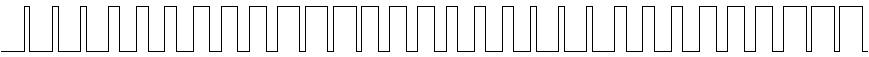
\includegraphics[width=\textwidth]{imgs/drawings/pwm/sinuois.png}
 \caption{The original sound.}
 \end{figure}
\par

\par
\begin{figure}[H]
\centering
 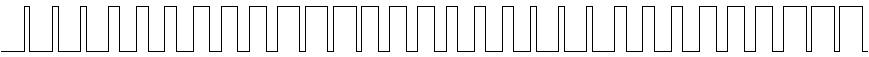
\includegraphics[width=\textwidth]{imgs/drawings/pwm/pwm_approximation.png}
 \caption{The same sound approximated with square wave and frequency changes.}
 \end{figure}
\par

To do this, the audio system once again relies on the PIT chipset. Counter 0 is used to trigger the audio system. Counter 1 is used to refresh the RAM periodically. Counter 2, however, is directly connected to the PC Speaker. The trick is to set this Counter 2 to square wave mode (Mode 3) so it will repeat after it triggers and program the desired square wave frequency. \\
\par
\begin{figure}[H]
\centering
   \begin{tabularx}{\textwidth}{ X X  }
	  \toprule
	  \textbf{Mode} & \textbf{Type} \\ \bottomrule
	    0 & Interrupt on Terminal Count\\
		1 & Hardware Re-triggerable One-shot\\
		2 & Rate Generator\\
		3 & Square Wave Generator\\
		4 & Software Triggered Strobe\\
		5 & Hardware Triggered Strobe\\
	  \bottomrule
  \end{tabularx}
  \caption{Available modes of a PIT counter.}
\end{figure}
\par 
When instructed to play a PC Speaker sound effect, the audio system sets itself to run at 140Hz via PIC Counter 0. Every times it wakes up, it reads the frequency to maintain for the next 1/140th of a second and writes it to Counter 2. The frequencies to use are encoded as a stream of bytes, the value of which is decoded as follows:\\
\par 
\begin{minipage}{\textwidth}
\lstinputlisting[language=C]{code/pwm.c}
\end{minipage}
\par
In the assembly, three I/O ports are accessed:\\
\par
\begin{minipage}{\textwidth}
\lstinputlisting[language=C]{code/pwm_code_header.c}
\end{minipage}
\par

While the end result was not great, it was better than a beep.\\
\par
\bu{Trivia :} LucasArts obtained surprisingly good results for their game Monkey Island. See the video "LGR - Evolution of PC Audio - As Told by Secret of Monkey Island"\footnote{https://www.youtube.com/watch?v=a324ykKV-7Y}.\\
\par
\begin{minipage}{\textwidth}
\lstinputlisting[language={[x86masm]Assembler}]{code/pwm_code.asm}
\end{minipage}
\par

Notice how the \cw{* 60} is not calculated but looked up. Once again the engine tries to save as much CPU time as possible by using a bit of RAM. The frequency is read from a lookup table \cw{pcSoundLookup}.\\
\par
\begin{minipage}{\textwidth}
\lstinputlisting[language=C,morekeywords=word]{code/pcSoundLookup.c}
\end{minipage}
\par
Notice how \cw{b6} (\cw{10110110}) is sent to the PIC Command register:
\begin{itemize}
	\item \cw{10} = Target Counter 2.
 	\item \cw{11} = High \& low byte of counter updated.
	\item \cw{011} = Square Wave Generator.
	\item \cw{0} = 16 bit mode.
\end{itemize}
\par











\subsection{PC Speaker: PCM}
\label{pcs_pcm}
The source code features an audio code path which plays PCM digitized sound via the PC Speaker. The function \cw{SDL\_PlayDigiSegment} has a switch to route playback. Notice the branch leading to \cw{SDL\_PCPlaySample} allowing PCM to be played on the buzzer.  \\

\par 
\begin{minipage}{\textwidth}
\lstinputlisting[language=C]{code/sound_fork.c}
\end{minipage}
\par
The problem of this method is to find a way to fit 8 bit samples into a 1 bit DAC. Let's take the example of the digitized sound "Mein Leben" which has 6,896 samples of 8 bits.\\




\begin{figure}[H]
  \centering
  \scaledimage{0.98}{audio/mein_liben.png}
  \caption{Mein Leben PCM 8 bit. You can clearly see the three syllables.}
\end{figure}
\par

The audio system goes for a surprisingly straightforward solution. It set itself to run at 7000Hz and manually move the cone of the speaker, using quantization to map 256 values to either 1 or 0.\\
\par
\begin{minipage}{\textwidth}
  \lstinputlisting[language={[x86masm]Assembler}]{code/pcm_on_speaker.asm}
\end{minipage}
\par
 \cw{SDL\_t0ExtremeAsmService} takes an 8 bit value and convert it to \cw{00} or \cw{10} to drive bit 1 in I/O port \cw{61h}. When bit 1 is set to 1, the beeper cone will go in position high and when set to 0, it will go to position low.\\
\par

\par
\begin{figure}[H]
  \centering
  \scaledimage{0.98}{audio/mein_liben_1_bit.png}
  \caption{Mein Leben resampled to 1 bit.}
\end{figure}
\par
The visual representation of a 1 bit per sample "Mein Leben" PCM looks like mashed potatoes but it sounds remarkably good. You can hear it thanks to a passionate YouTuber named Dafe Allen who recompiled the engine with PCM playback enabled\footnote{"Wolfenstein 3D Hack - Digitized PC Speaker Sound Effects": "https://www.youtube.com/watch?v=1BtlsjJRnFU".}.\\
\par
As good as it sounds, this codepath shipped but was never enabled. According to John Carmack overhead was too much a problem. Jim Leonard provided a more in depth explanation.\\
\par

 \begin{fancyquotes}
 PCM playback over the PC speaker was likely cut because it would require SDL\_t0ExtremeAsmService. The Disney Sound Source had a 16 byte buffer but the PC Speaker had no such thing, the only way to feed it fast enough is to run the interrupt audio system at 7000 Hz.\\
 \par
  High-end 386s could handle this, but this was nearly unsustainable on the 286. Sending data to the parallel port does not take a lot of time -- but interrupt overhead does, and 7000 Hz on a 12 MHz 286 would definitely have been noticeable.\\
 \par
 Running at a frequency this high would have caused the game to freeze on slower machines while the sample played through the speaker.\\
\par
 Jim Leonard
\end{fancyquotes}\\
\par









\subsection{PC Speaker: PWM}
Even though this method was not used in Wolfenstein 3D, it is worth mentioning a third way hackers managed to play pleasant sounds via the PC speaker. The method produced audio quality superior to both the square waves and the 1 bit conversion we just saw. It was called Pulse Width Modulation.\\
\par
The idea is to manipulate the speaker cone manually and instruct it to move faster than it can, interrupting it "somewhere" between its position up or down.\\
\par
The technique was patented (US US5054086 A) by Access Software and called RealSound. Many studio licensed it during the 80s but the advent of dedicated sound cards with FM and PCM capabilities made RealSound obsolete in the early 90s.
\par
 \begin{fancyquotes}
  The PC speaker is normally meant to reproduce a square wave via only 2 levels of output (the speaker is driven by only two voltage levels, typically 0 V and 5 V). However, by carefully timing a short pulse (i.e. going from one output level to the other and then back to the first), and by relying on the speaker's physical filtering properties (limited frequency response, self-inductance, etc)., the end result corresponds to intermediate sound levels. This effectively allows the speaker to function as a crude 6 bit DAC, thereby enabling approximate playback of PCM audio.\\
  \par
  This technique is called pulse-width modulation (PWM).\\
  \par
  Jim Leonard - oldskool.org
 \end{fancyquotes}
\par
In the next drawing we see how commanding the cone faster than it can move results in intermediate positions.
\par
\begin{figure}[H]
  \centering
  \includegraphics[width=\textwidth]{imgs/drawings/pwm.pdf}
  
\end{figure}
\par





